\section{Technical Development}
\subsection{User Interface Design}
The User interface for this project is designed after looking at the user interfaces used by other music applications. In particular, the developer was inspired by Spotify, shown in figure \ref{fig:spotify}.

\begin{figure}[h]
    \centering
    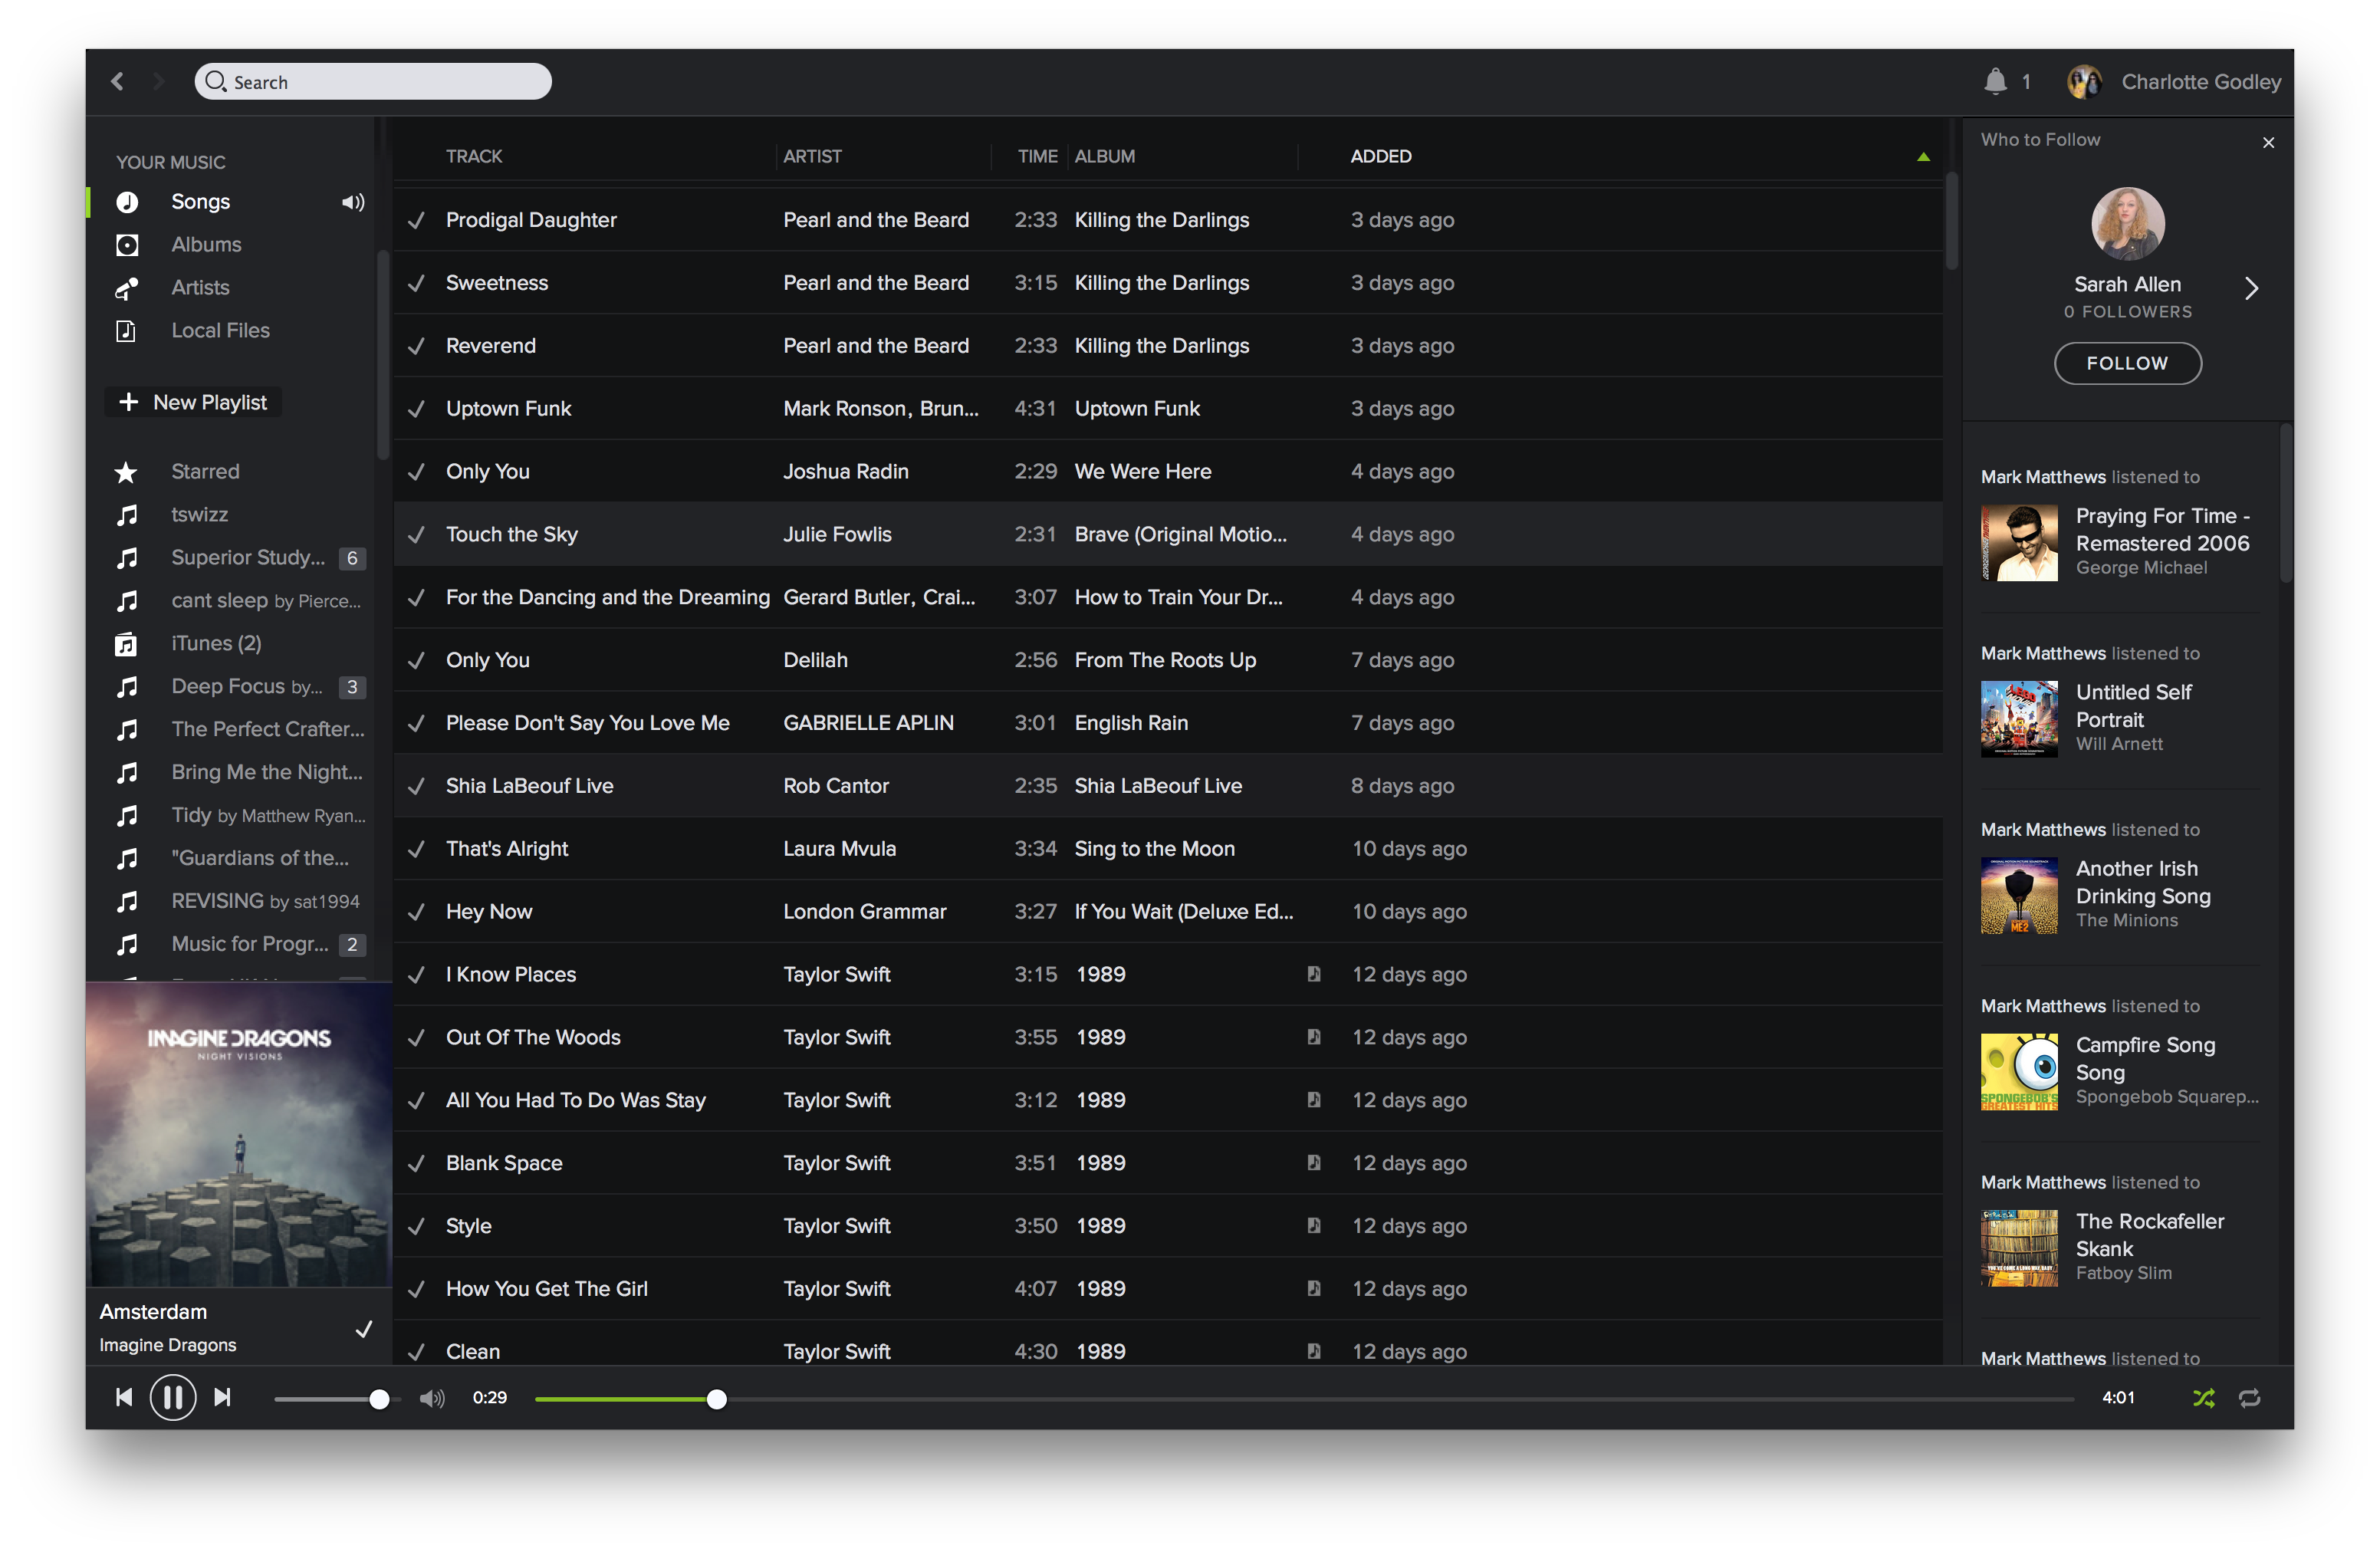
\includegraphics[width=\textwidth]{screen.png}
    \caption{Spotify user interface}
    \label{fig:spotify}
\end{figure}
\subsubsection{Main Display}
\begin{figure}[H]
\centering
    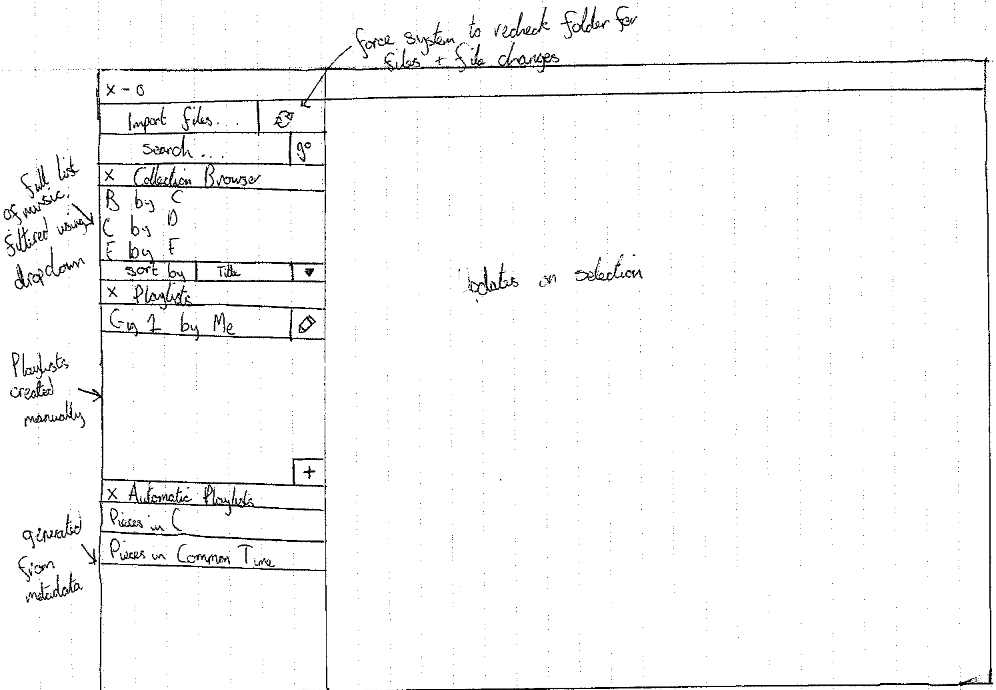
\includegraphics[width=500pt]{designs/main}
    \caption{Main User interface of the project - design}
    \label{fig:main_handdrawn}
\end{figure}
Figure \ref{fig:main_handdrawn} shows the main view of the application. The developer took this design and the other hand drawn designs which are in the appendix and produced a prototype using QtDesigner. The main window produced using this system and linked to the application is shown in figure \ref{fig:main}, updated to show details about the sheet music displayed in the PDF window. 
\begin{figure}[H]
	\centering
    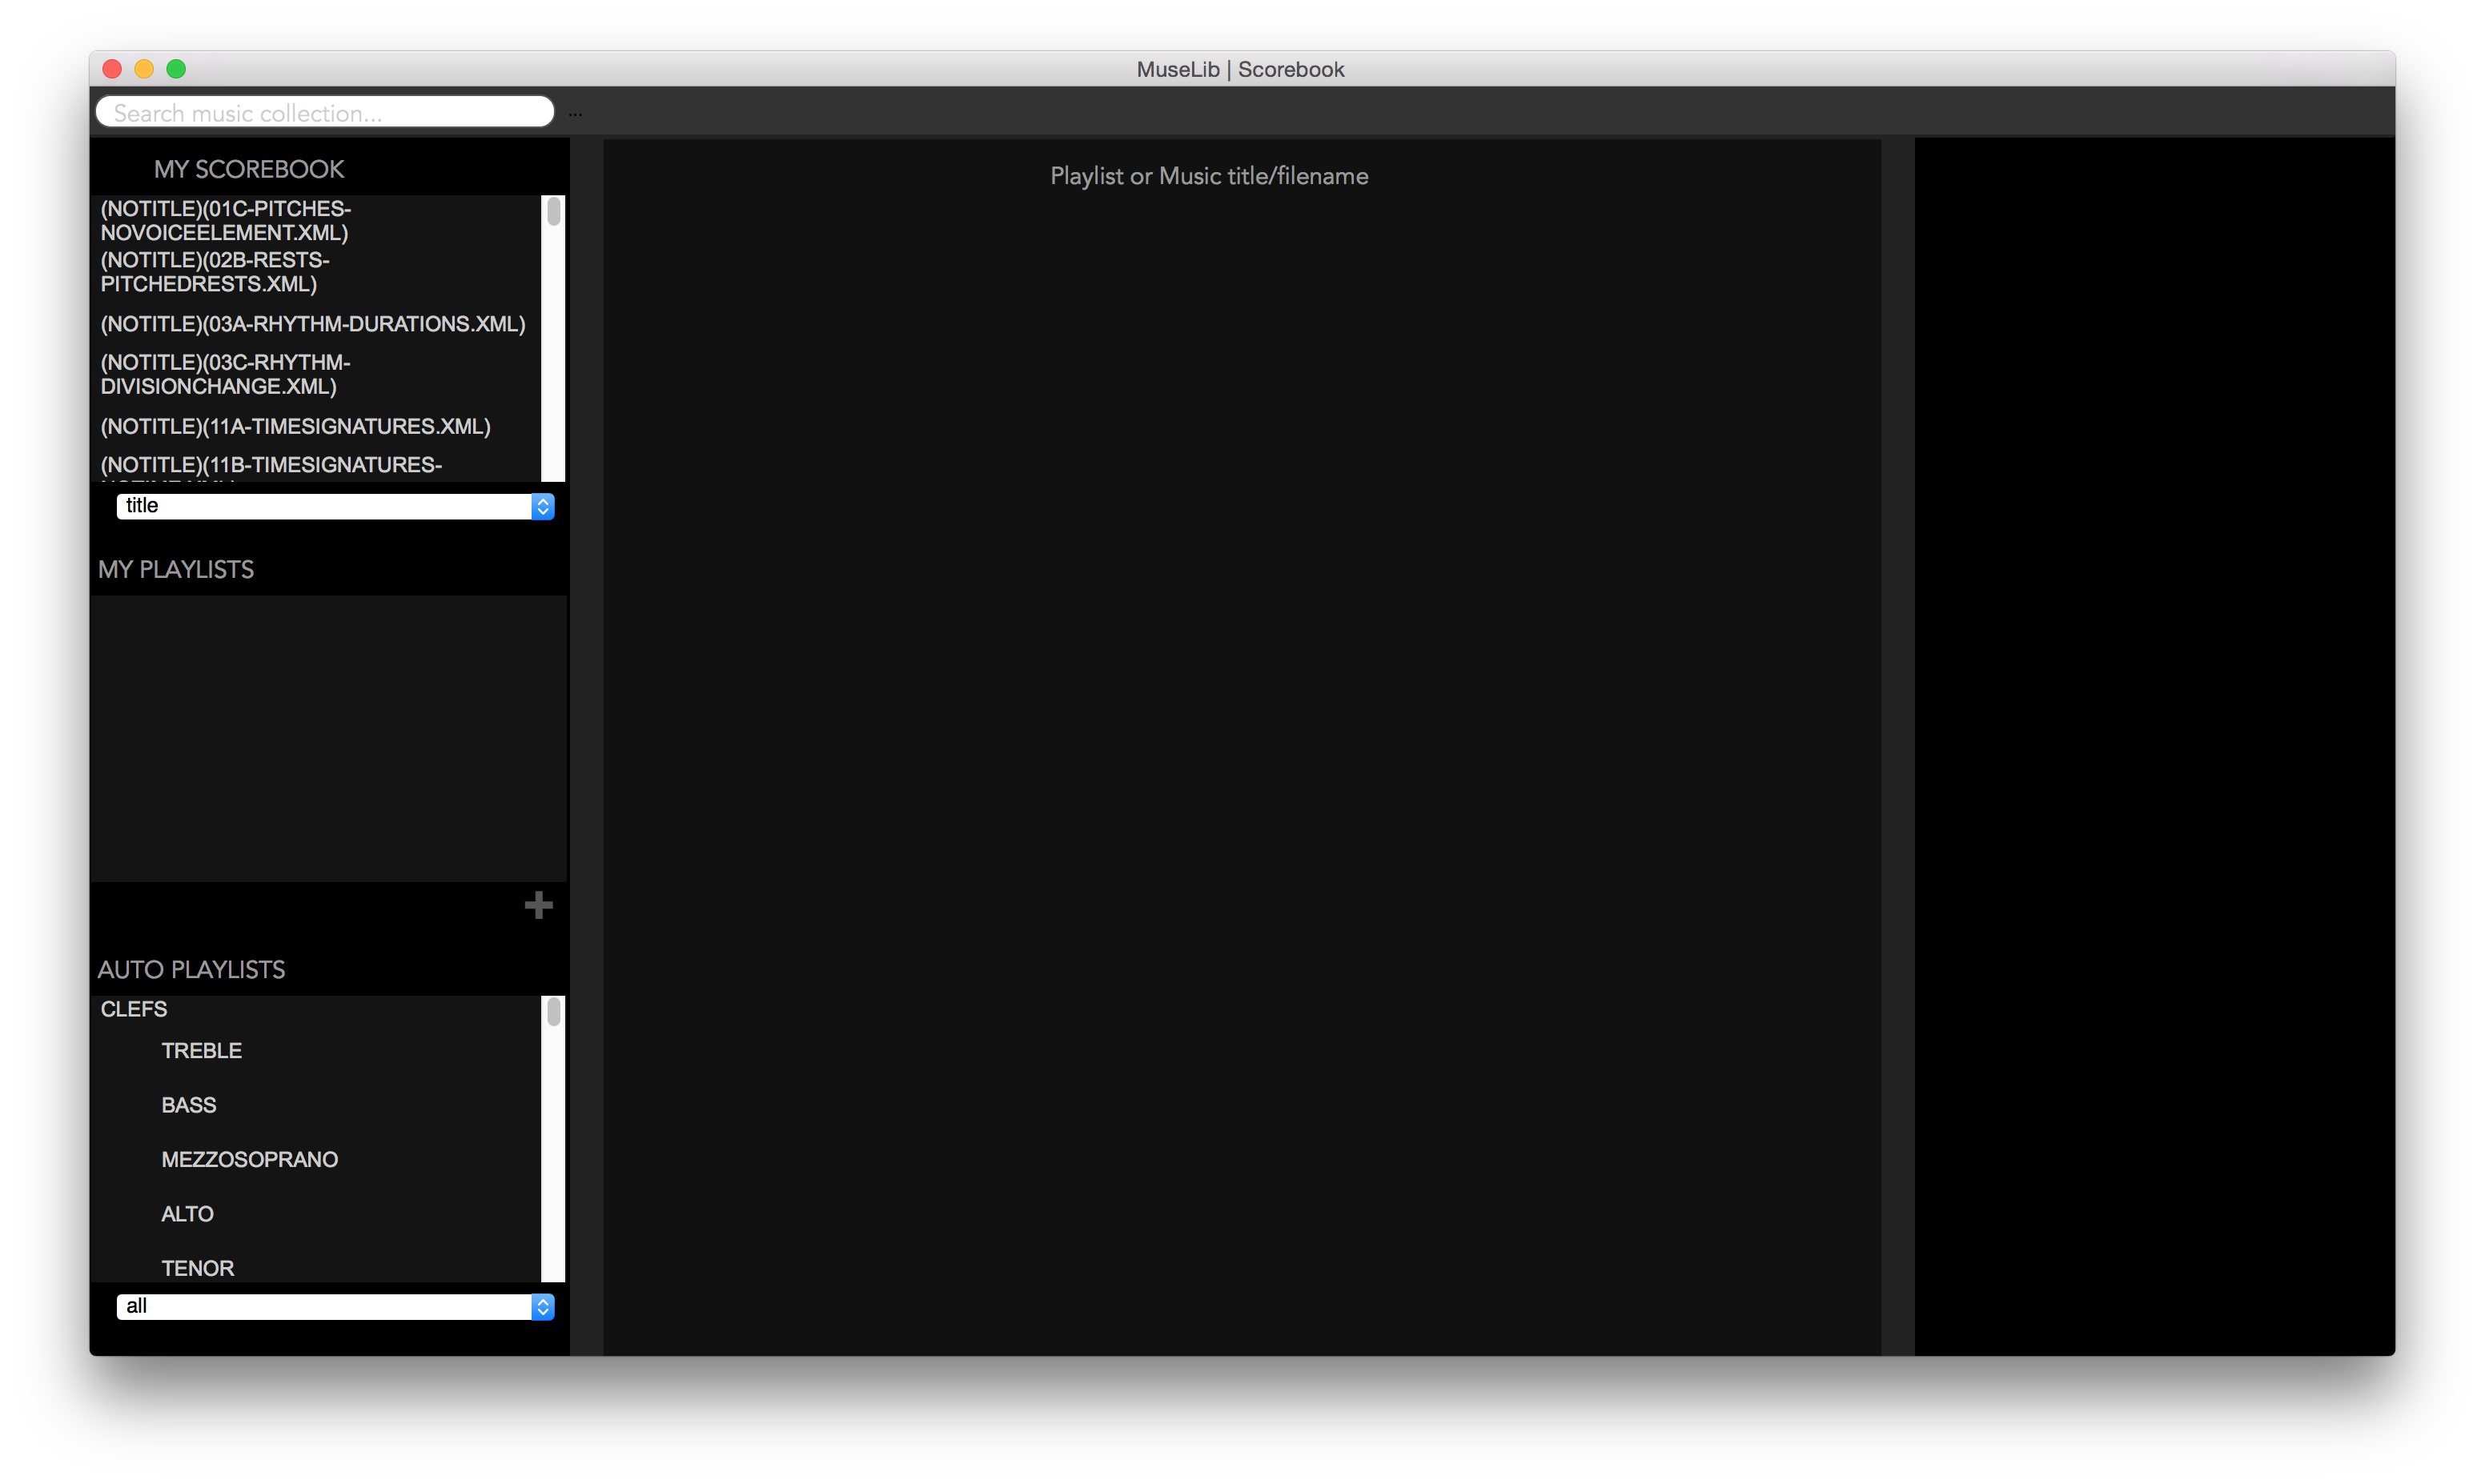
\includegraphics[width=400pt]{designs/main_screenshot.png}
    \caption{Main User interface of the project - implementation}
    \label{fig:main}
\end{figure}
All of the frames of the user interface are styled using a CSS stylesheet, so that the developer could customise everything with precision. This also meant the developer could easily implement a light theme, as shown in figure \ref{fig:main_light}. The remaining screenshots and explanation of how different windows link together are given in the user guide, which is in the appendix.

\begin{figure}[H]
	\centering
    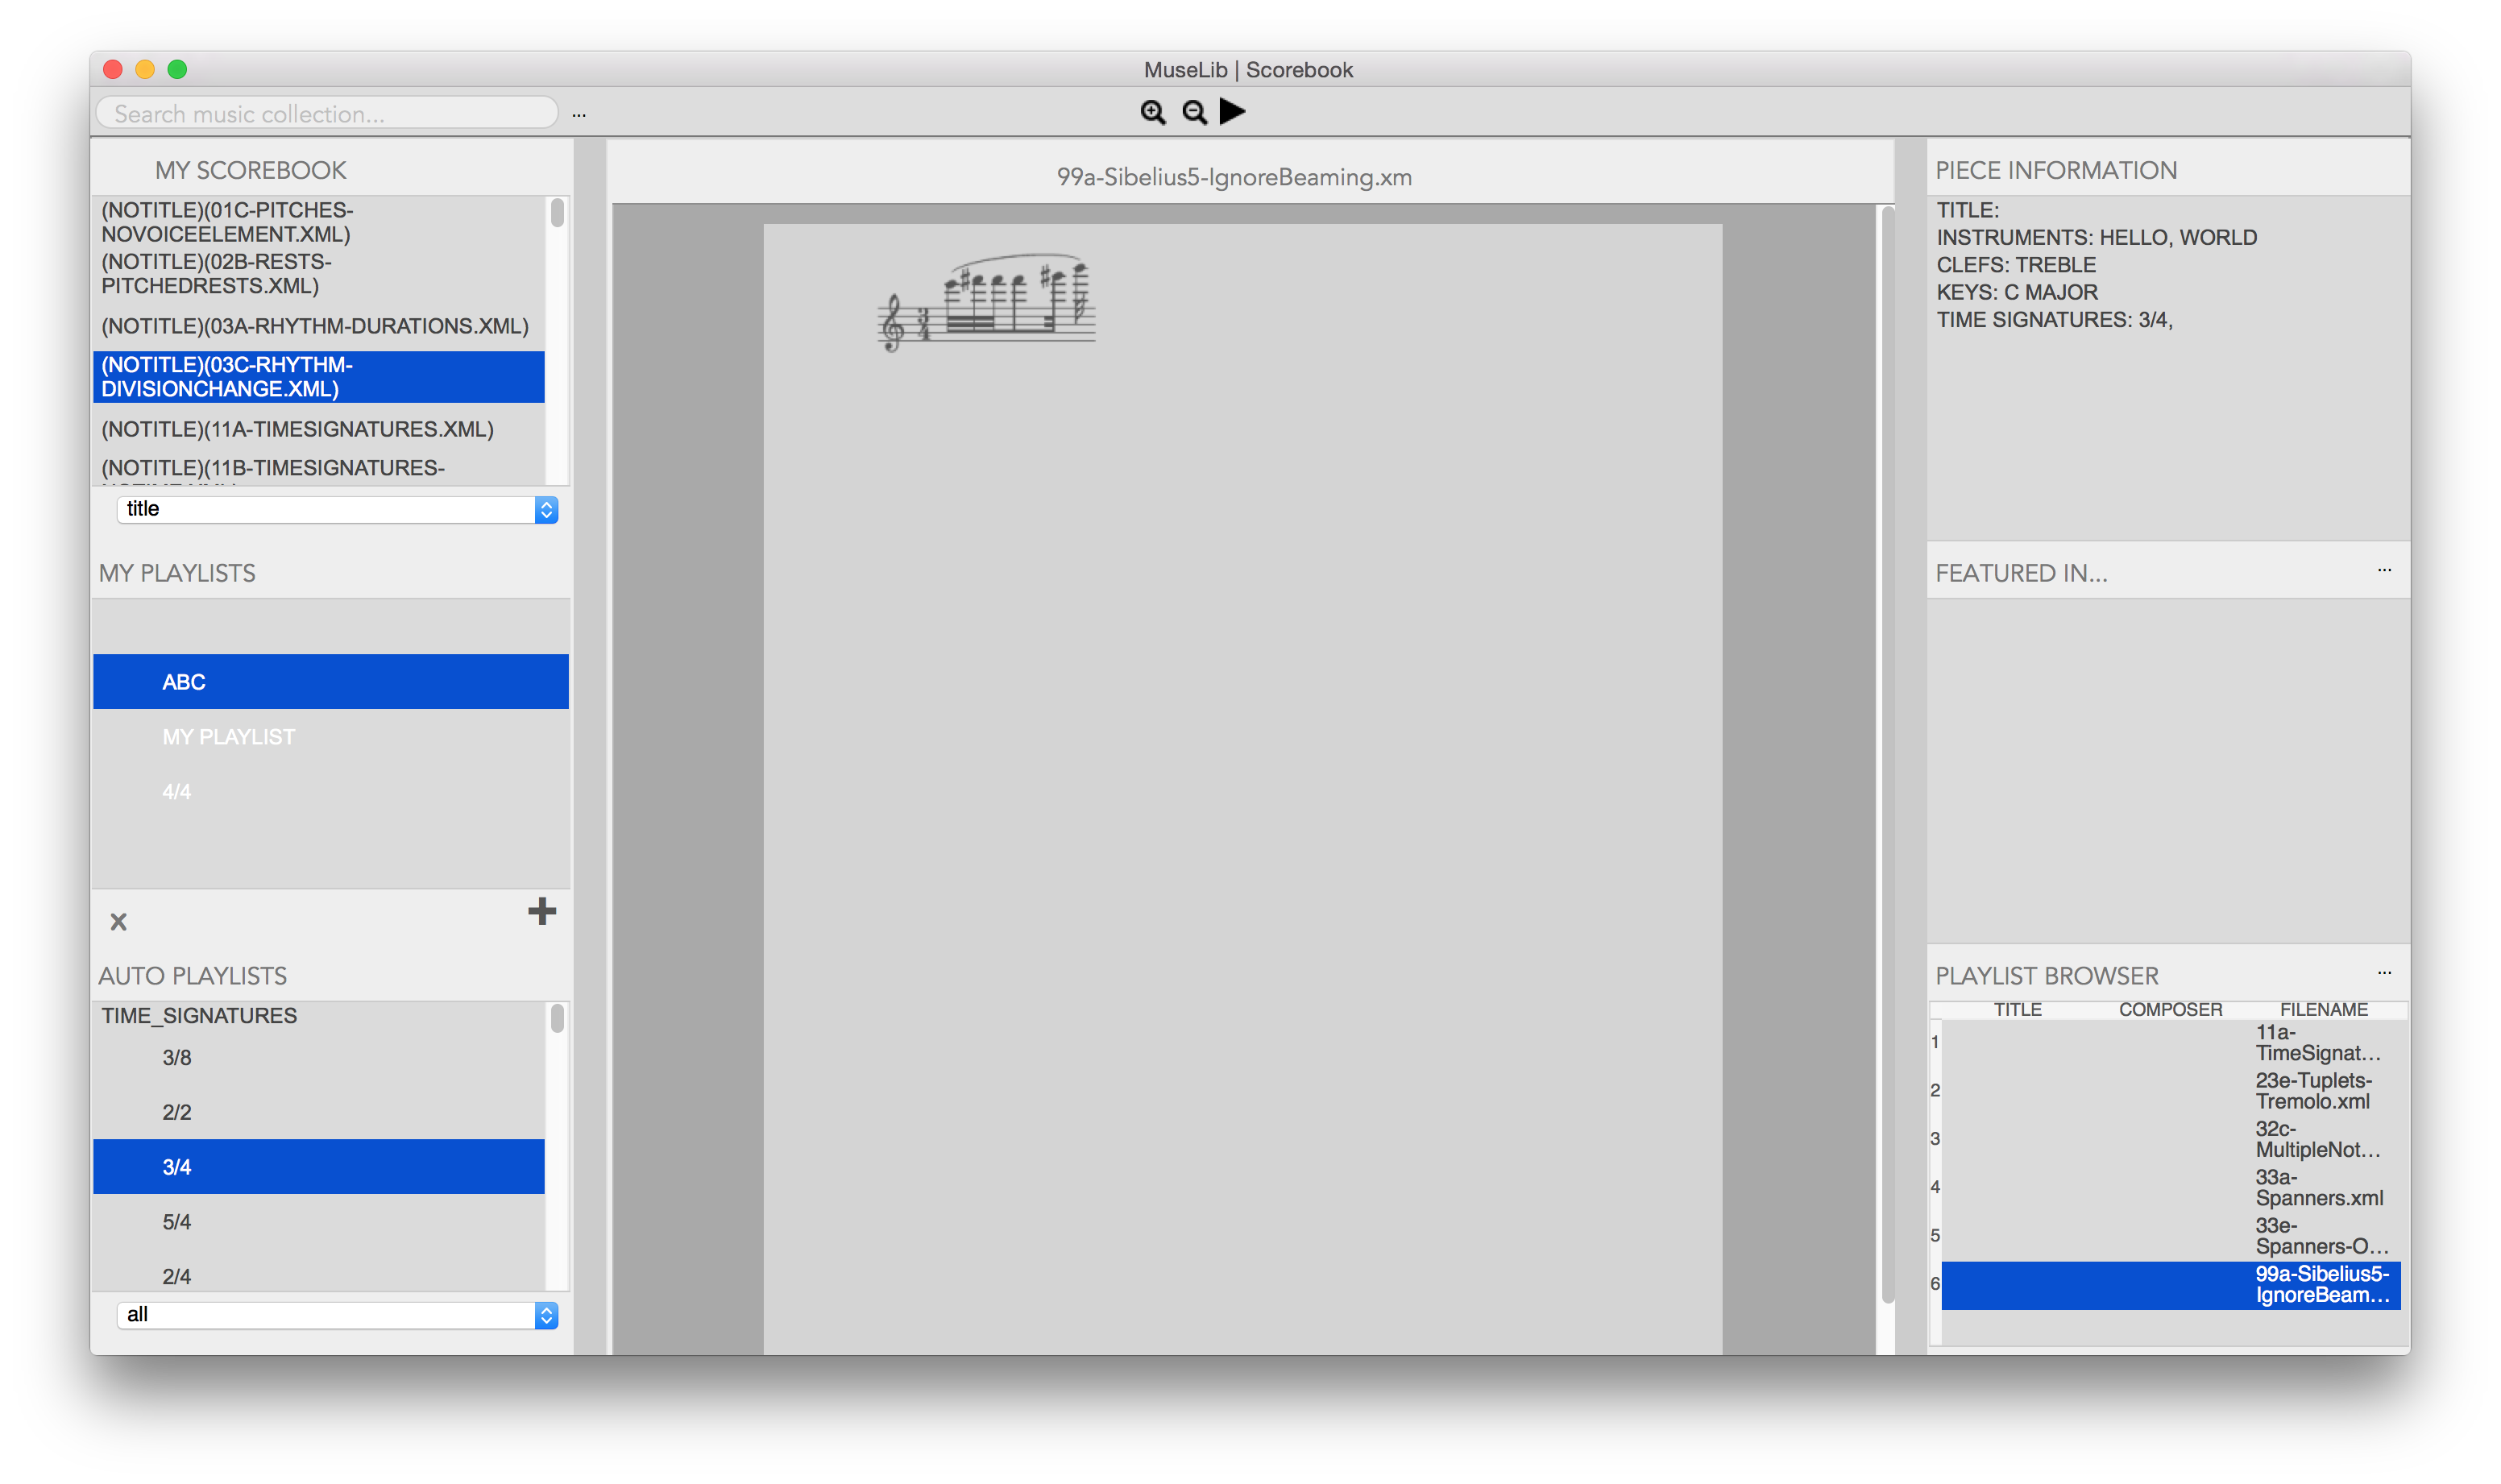
\includegraphics[width=400pt]{designs/main_light.png}
    \caption{Main User interface of the project - implementation: Light Theme}
    \label{fig:main_light}
\end{figure}
\subsection{Test Design and System Testing}
\subsubsection{Test Driven Development}
This project was developed using Test Driven Development. This is an Agile software development methodology which utilises the rules that a line of code should not be written unless there is a failing automated test \parencite{TDD}. This methodology has been chosen as the nature of the notation of music means that meticulous attention must be paid to how and with what symbol every element is notated, and Test Driven Development will significantly improve the quality of the software by closely integrating testing with the development process.

As such, no test design or plan was produced, but rather tests were developed as features were introduced, and were designed to be self contained units testing the smallest possible details, such as an accent being added to a measure correctly, or a note's pitch being created with a particular note name or octave number.

\subsubsection{Unit Testing}
Unit tests for this project were created on an objective by objective basis using the standard python unit tests testing suite. The developer's IDE of choice, Pycharm, has built in support for this module, with an intuitive interface for running tests in a given file and production of readable output of what happened in each tests, as shown in figure \ref{fig:testing_interface}.

\begin{figure}[h]
	\centering
	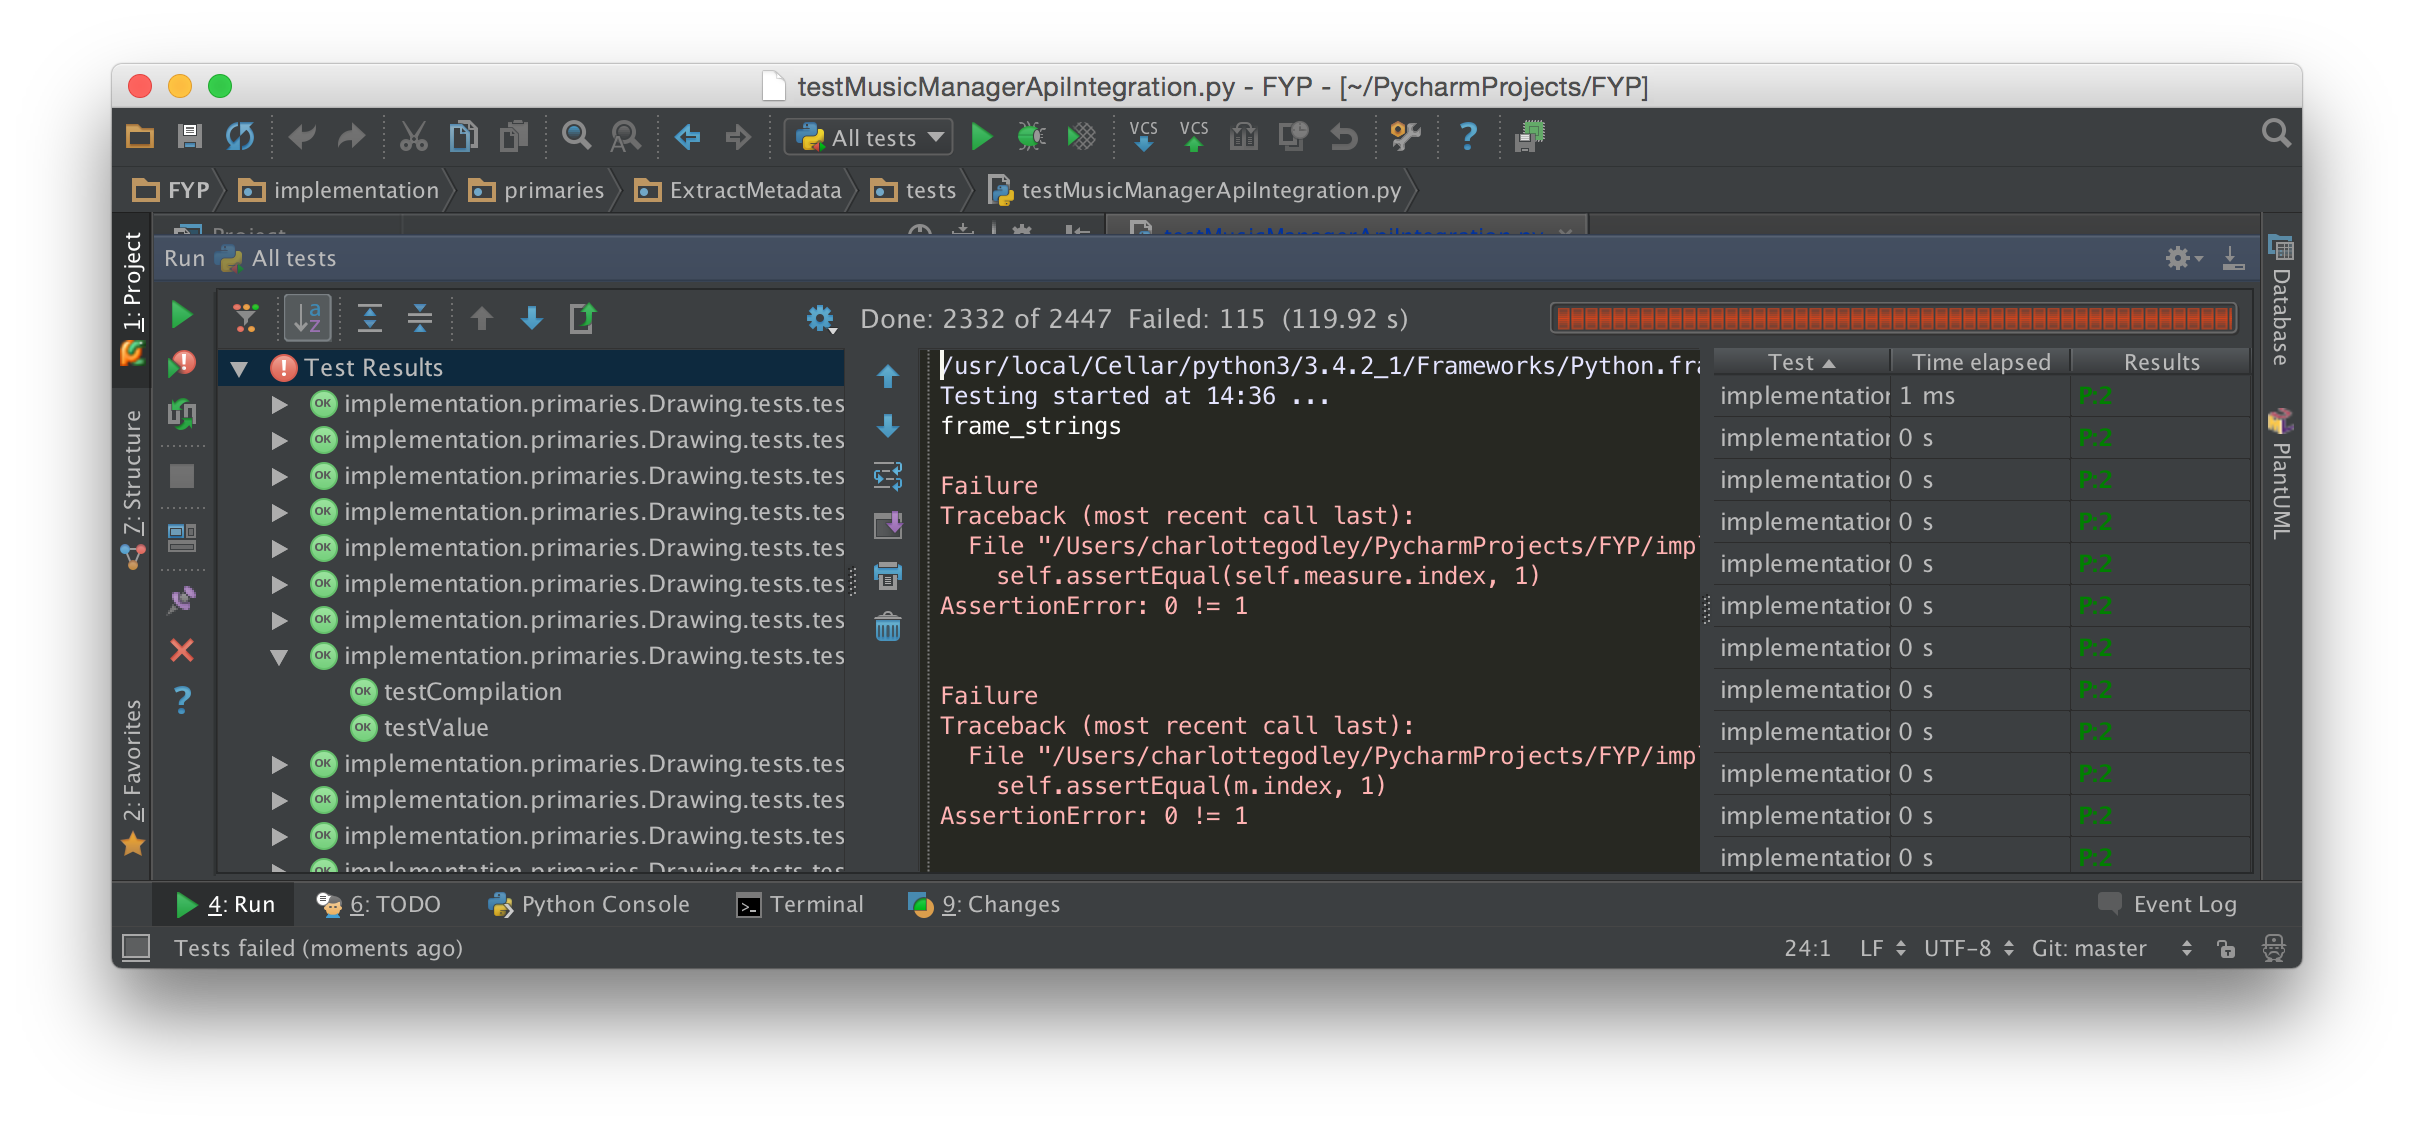
\includegraphics[width=\textwidth]{testing_interface}	
	\caption{An example of testing integration in PyCharm}
	\label{fig:testing_interface}
\end{figure}

The interface also includes the ability to create scripts which discover and run tests on folder, file, class and method level, as shown in figure \ref{fig:testscript}. The developer used this feature to create scripts which ran all of the tests for specific areas of each objective, as well as the objective itself. This enabled the developer to quickly check new features had not affected the status of previous features. 
\begin{figure}[H]
	\centering
	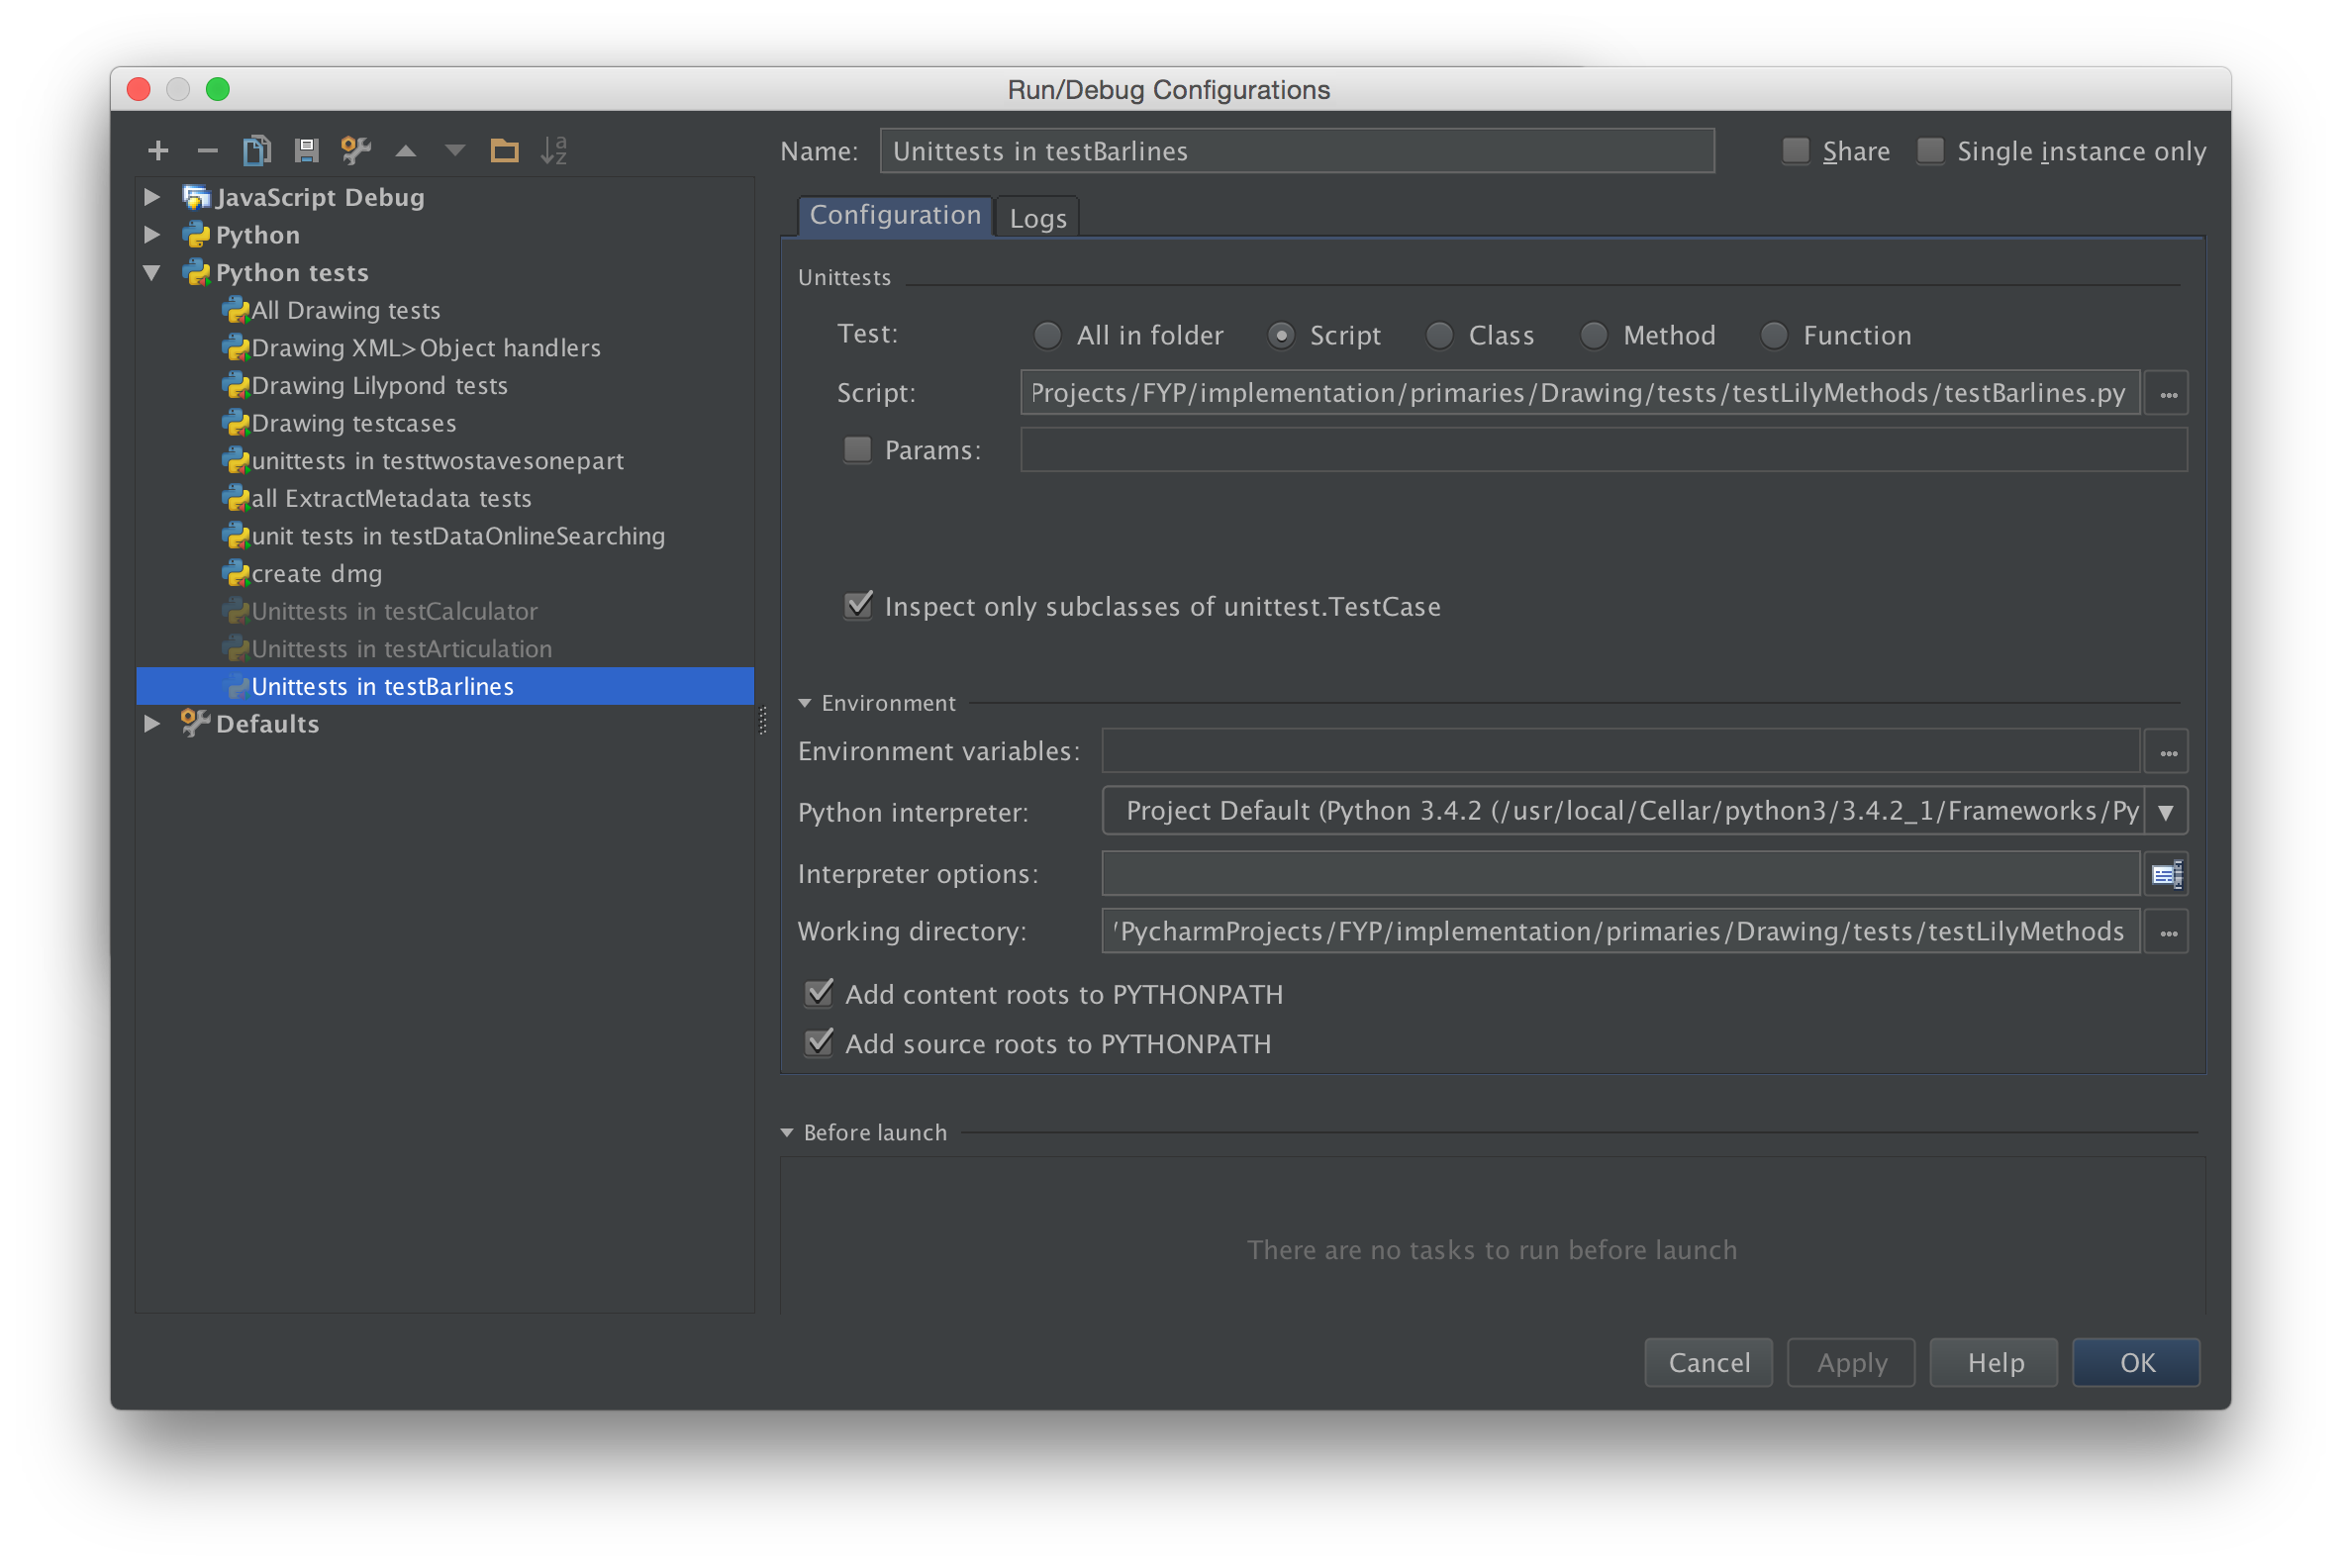
\includegraphics[width=\textwidth]{create_test_script}	
	\caption{An example of script creation in PyCharm}
	\label{fig:testscript}
\end{figure}
\subsubsection{Unit Testing the rendering system}
In the initial phase of developing the rendering system, the SAX parser was tested at base functionality level, with checks that new tags, new data and closing tags modified various lists which handler methods used to extract information. As new functions and tags were handled, more and more tests were developed for every tag, termed handler tests. These tests included combinations of tags and combinations of tag attributes, as well as testing tags in exclusion from other tags. When new features were introduced the developer would run the full set of unit tests before committing the code to source control, in order to ensure that new features did not cause regressions or changes in previously developed code.

When the object extraction algorithm portion of the rendering system was completed, the developer created unit tests for the individual symbol classes to confirm their ToLily method worked according to what was expected in the lilypond documentation.

Once the individual symbols were tested, the developer created tests to check the classes containing the symbols concatenated the strings of output in the correct order. As every possible value and change to each symbol had been tested at symbol class level, this portion of testing was not as extensive and only included tests to confirm ordering of notes, directions and expressions were valid where they had any effect on each other. For example, it would be unnecessary to test a note with every possible dynamic marking, but it was necessary to test a dynamic did not occur before a note.


\subsubsection{Development of Test cases}
In order to test the system more extensively, the developer created several MusicXML test cases. A full list of the test cases used is given in the appendix, as well as a sample file. In order to produce the test cases the developer used the composition software MuseScore, and systematically went through each category of symbols provided producing every possible type of symbol for that category. These were saved as individual files, titled by each category of symbol.
The developer then produced unit tests which checked the object hierarcy when the parser loaded the file. Each test and test method confirmed that the objects were in the right place within the piece, part and measure, and that each object had the appropriate values.

Once the lilypond output section of the objective was completed, the developer reused the test cases to check their lilypond output. Initially, the tests were primitive, only confirming that a pdf file with the same name had been created. Later, the developer produced an expected output lilypond file and checked the output of the test against the expected output.

\subsubsection{Use of Third Party Test cases}
As there was no official test suite available for MusicXML, the Lilypond project released an unofficial collection of music xml files for testing purposes \parencite{LilypondTestcase}. Each file tests individual elements of music xml, sometimes in collaboration with other areas. In total the test suite contains 131 files and represents the most comprehensive test suite currently available openly.

The developer ran the rendering system against each test case in the suite. Initially, the developer ran them individually, visually checking the output against the images in the documentation for the test suite, and then moving test cases which passed to a separate folder from the remaining test cases. Later, an automated script was created to attempt to speed up the process, though visual checking of the output was still necessary as no lilypond files were provided with the xml files.

Due to time constraints, the developer prioritised failures according to severity, which had three levels. The first level was failure to produce a lilypond output due to an exception in the program. The second level was failure to produce a pdf output due to the lilypond output being invalid. The third and final level was failure to produce a pdf output which matched the expected output. Each failure in any sense was reported using the issue tracker on Github, with an indication of the filename which failed as well as the reason for the failure. An example of such an issue report is given in figure \ref{fig:issue}.

The developer ensured that all test cases were above the first two levels of severity, and then made a decision on how important the symbol was in the context of it's usage in western music, as well as the time remaining to work on the other two primary objectives.

At the point of stopping work on the rendering system, 65$\%$ of the test cases in this suite passed and produced the correct graphical output. 
\begin{figure}[H]
	\centering
	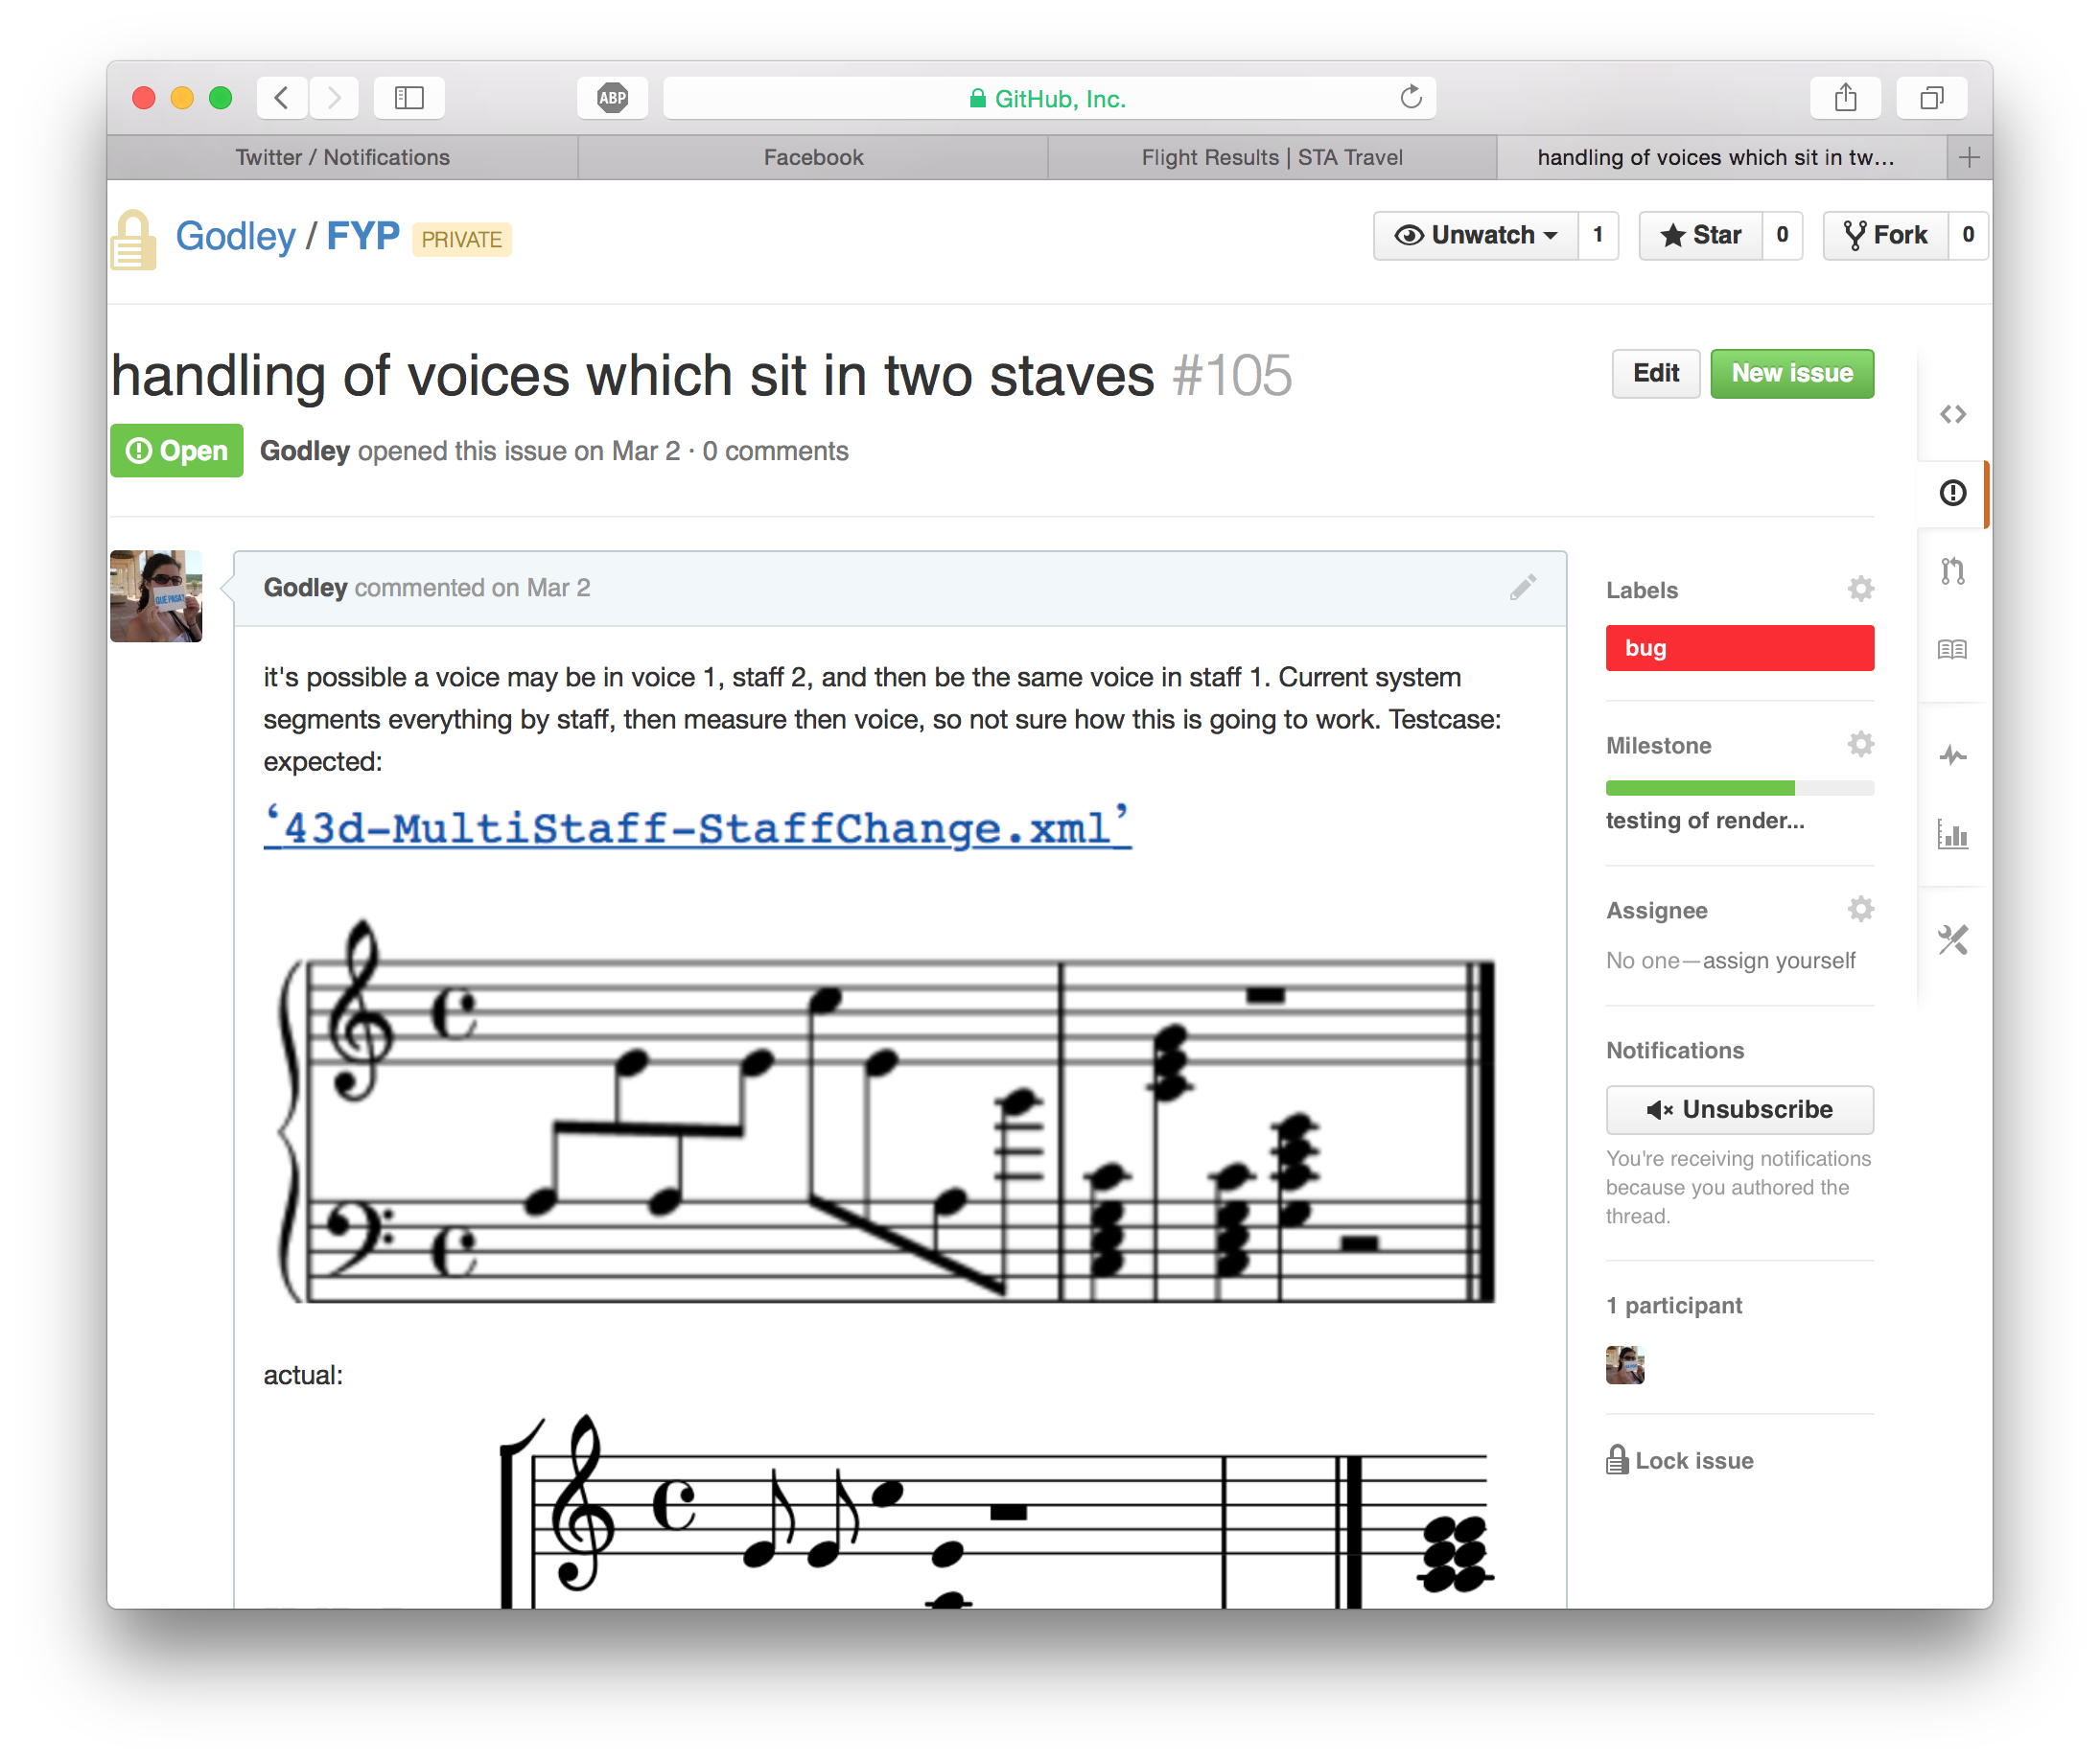
\includegraphics[width=400pt]{issue_report}	
	\caption{An example issue report}
	\label{fig:issue}
\end{figure}

\subsubsection{Unit testing the metadata and API objectives}
Unit tests were written for the other two objectives in a similar way to the rendering system.

For the metadata scanning objective, the developer tested each element of the system in exclusion from each other. This divided the process into four classes, the folder browser, the unzipper, the data layer, and the metadata parser, as visualised in the class diagram in figure \ref{fig:metadiagram}. One main class, the music manager, handles the connections between each element. Like the rendering system, this meant that the tests for combining the elements together did not need to be so complicated as the functionality of each element had been tested rigourously.

For the online collections objective, tests were created at source API class level, then API manager level, and finally the API manager was tested when integrated with the music manager class.

\subsection{System Design}
\subsubsection{Overall Architecture}
The flow chart in figure \ref{fig:flowchart} was designed in the initial prototype phase in order to visualise how the objectives would interlink with each other.
\begin{figure}[H]
    \centering
    \includegraphics[width=400pt]{diagrams/overall_system.pdf}
    \caption{A flow diagram describing the project}
    \label{fig:flowchart}
\end{figure}

\subsubsection{Metadata Scanning system}
The flow diagram in \ref{fig:flowchart} refers to applying a metadata scanning system to the folder. This is described in more detail in the flow diagram in figure \ref{fig:meta}. 
\begin{figure}[H]
    \centering
    \includegraphics[width=250pt]{metadata_algorithm-crop}
    \caption{A flow diagram describing the meta scanning system}
    \label{fig:meta}
\end{figure}
\subsubsection{Metadata Class Structure}
The metadata scanning objective implements the popular Model View Controller design pattern, which separates the user interface (view) from the program logic (controller) and any databases or information storage (model) \parencite{mvc}.
In this instance, as shown in the class diagram in figure \ref{fig:metadiagram}, the music manager class acts as the controller, which takes input from the application interface. The music manager processes the input and turns it into requests for data, which are sent to the data layer. The data layer communicates with an SQLite file containing several tables, and sends collections of requested data back to the music manager, which updates the user interface with the new information.

The decision was taken to use this pattern in order to avoid coupling to any particular database and to ensure that the objective was properly organised according to functionality. The decision was also influenced by considerations about the future of the project, including expansions to include online data layers or improvements to the UI without affecting program logic.

\begin{figure}[H]
    \centering
    \includegraphics[width=\textwidth]{diagrams/api_and_meta_data_diagram}
    \caption{Metadata and API Class Diagram}
    \label{fig:metadiagram}
\end{figure}

\subsubsection{Modular Design}
The MVC design pattern was complemented by the implementation of the  modular design pattern, in which functions and collections of functions are separated into independent blocks or modules \parencite{modular}.

This is shown in the class diagram in figure \ref{fig:metadiagram} as the music manager also interacts with other classes such as the folder browser, which handles all functionality involving scanning the given folder for new, old, or zipped files, and the unzipper, which handles the functionality for manipulating zip files.

It is also present in the rendering system explained in detail in section 4.3.5, as each section of the object hierarchy collects its own Lilypond formatting, and then calls upon its child classes to collect theirs, finally collaborating into one complete Lilypond file. In the context of sheet music this is particularly important, as symbolic notation has many options for symbols which may or may not be present, so in program logic they must all act independently of other symbols occurring in the file.

This design was influenced by the decision to use test driven development, as this development methodology aims to test small units of program functionality in an isolated environment \parencite{TDD}.
 As such, this was easier to achieve if each independent class had one role in the system, with management classes handling the collaboration of these roles without needing to test multiple elements of functionality at once. 

This makes the code and overall architecture reusable in different situations. For example, the API manager class sends data collected online back to the Music Manager, which can then communicate with the metadata scanner to extract further information, which avoids code duplication.

\subsubsection{Rendering Architecture}
The class diagram in figure \ref{fig:classdiagram} shows an abstract structure of the sheet music rendering implementation used in this project. This implements a tree, each node of which holds an item containing the notation specific to that node. Each node object implements the ToLily method, which generates a string of Lilypond formatted output representing itself and then calls each of its child nodes in turn for their outputs, combining them into one string. 

A tree was chosen as the object structure in order to give an indication of time, and in order that specific elements could be positioned according to sequential instructions from the MusicXML parser. 
\begin{figure}[H]
    \centering
    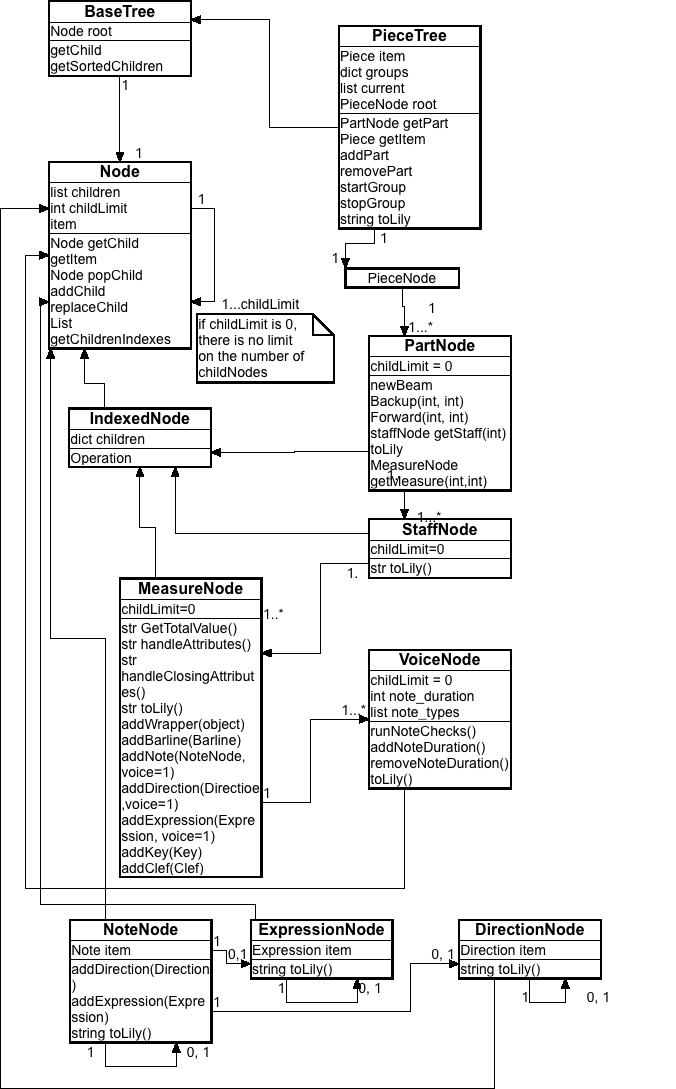
\includegraphics[width=250pt]{diagrams/render-tree.png}
    \caption{Renderer Class Diagram}
    \label{fig:classdiagram}
\end{figure}
\subsubsection{Duck Typing}
The rendering system visualised by figure \ref{fig:classdiagram} implements a feature of dynamic typing known colloquially as Duck Typing. Duck Typing is a method of type inference by which the program assumes that an object is of one type according to the behaviours that it has, not the exact type or attributes it may or may not contain. %todo ref

In respect to the rendering system, this means that each class assumes any child classes present will have the ToLily method, call the method and collaborate the results. Using this method of type inference is important to the project as this avoids assumptions about what the music will or will not contain, and instead defines that symbol as suitable for inclusion if it has the ToLily method. 

Implementing objects and program functionality using duck typing also means that future feature implementations or symbols which are added to the renderer need only implement a ToLily method and be linked into the input parser scripts in order to be implemented in the rendered output, and can be of any type the developer defines.

\subsubsection{Designing for extensibility}
The project is designed with a particular aim of extensibility. This affects each area of the system in a different way, but in general, it means that the elements in the system are able to be modified, improved or expanded without requiring changes to the organisation of the system. 

An example of this is the API manager, which holds a dictionary of sources, with each index pointing to a class. The API manager will cycle through these sources when its methods are called, meaning that to implement a new API, the developer would simply put a new entry into this dictionary.

Each source implements the API class. To avoid causing problems with classes missing particular methods, the API class will throw a not implemented exception if the sub class does not override the method, in order to indicate to the developer working with a new API that this method is necessary.

\subsubsection{Difficulty Rating input from users}
When considering the difficulty rating objective for this project, the developer was aware of the subjective nature of sight reading and rating. To assess how this varied from instrument to instrument, the developer produced a survey which was given to a wide range of musicians, as shown in figure \ref{fig:survey_difficulty}. The results of this survey are given in the appendix.

\begin{figure}[H]
\centering
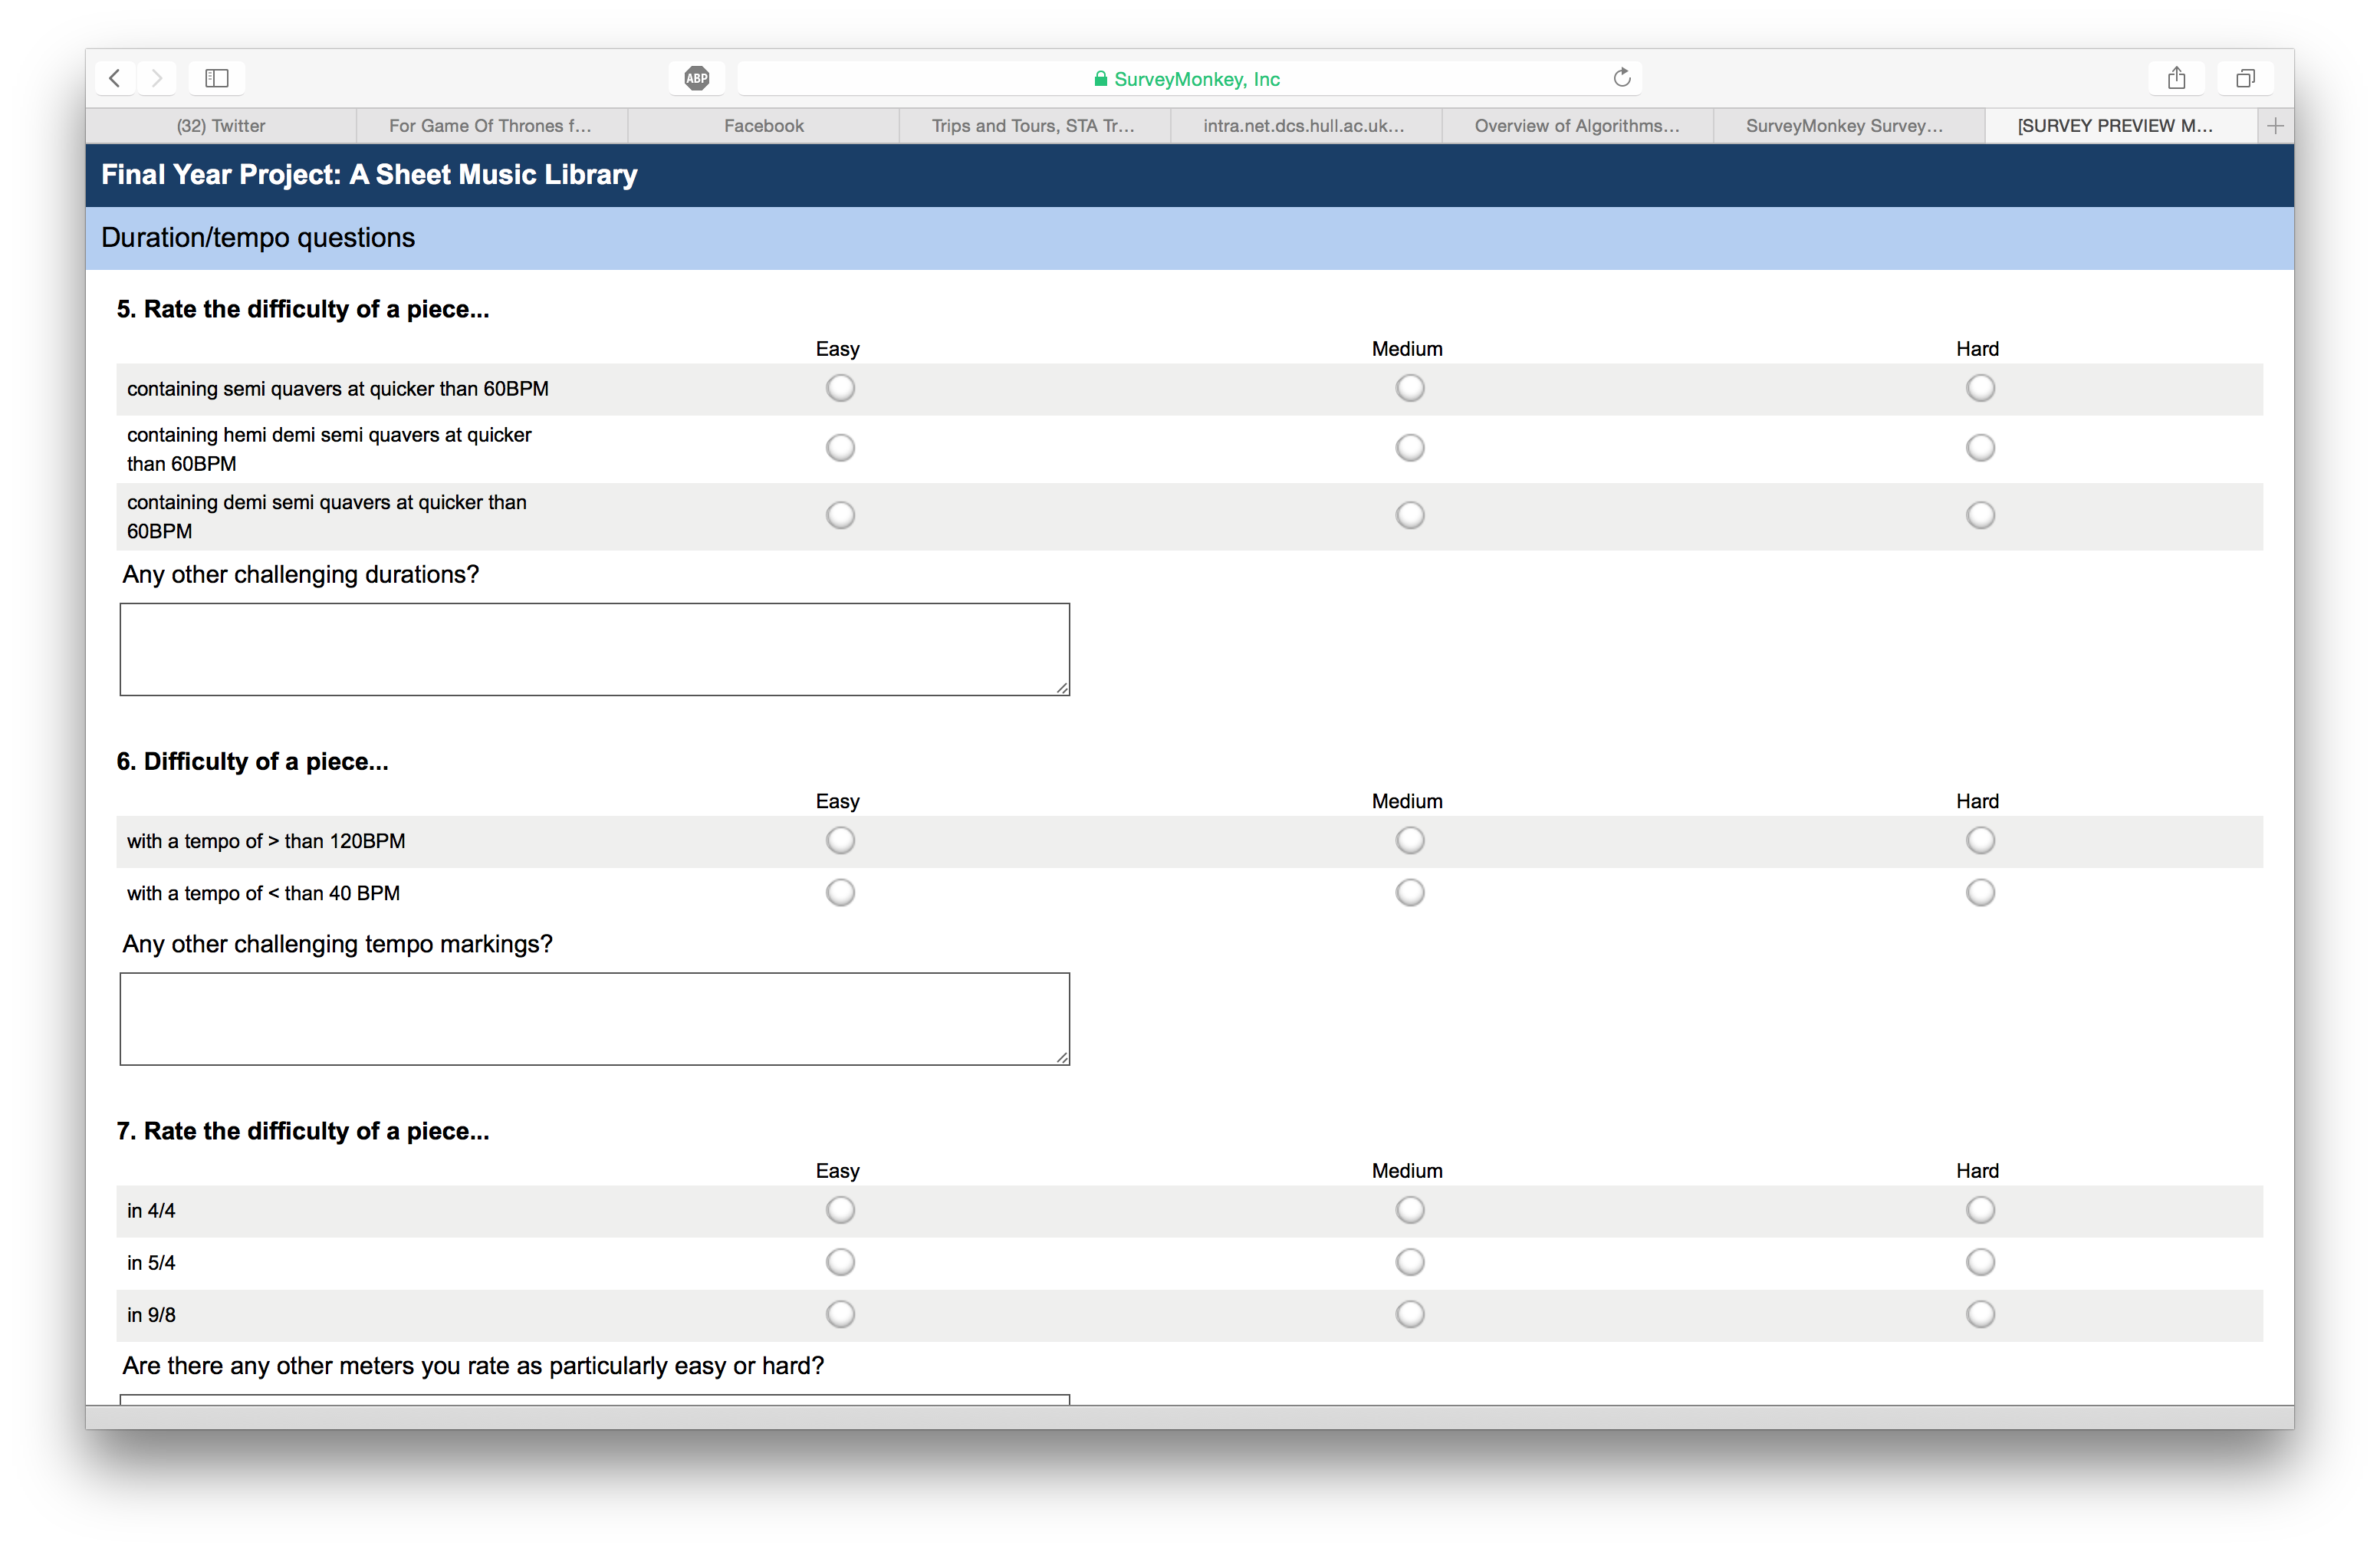
\includegraphics[width=400pt]{survey_difficulty}
\caption{An online survey on piece difficulty}
\label{fig:survey_difficulty}	
\end{figure}



\subsection{System Implementation}
\subsubsection{Development Methodology}
The project was implemented using a developer informed process. In this process, the developer would review the project's status for bugs, issues and features which had yet to be implemented and note this using the Github Issue Tracker. When the developer began working with the code, they would select an issue based on the priorities of the project, develop tests for this issue and finally, develop the production code and close the issue.


Issue tracking and reporting was used so that the developer could think and reflect on areas of the system which needed improvement, modification or implementation. The methodology worked well in the context of a year long project in which development was not continuous because it ensured that when development was paused, the developer could see instantly what needed to be doing or what was being worked on before the pause to work on something else. 

This adds the benefit that in the future, when this project may be worked upon by more than one developer, new developers can see things which have yet to be implemented and choose which features are most relevant or doable by their own standards, as well as discuss or contest previous issues in the system.


\subsubsection{Challenges in the rendering system}
The renderer in this project was designed around two open formats - MusicXML and Lilypond. Whilst every effort was made to avoid coupling with either format, designing the system to work seamlessly with both formats was difficult, and many problems were encountered structuring the object format.

Initially, the project used a simpler object structure in which measures contained a list of items contained within that measure. The decision was taken to use lists of items loaded sequentially becase MusicXML items have no unique identifiers which could be used to indicate at which point they occurred within that measure, so objects had to be loaded and stored sequentially.

It was then discovered that Lilypond dictates that dynamics and some other elements, which are classed as directions in MusicXML, had to occur directly after the note to which they should be assigned \parencite{ExpressionLilypond}.
 The structure had to be redesigned based on this information in order to classify notes as first class objects, for which other elements would be indexed according to which note they occurred after, and that directions and expressions needed to be split into two lists, in order to ensure that expressions could be put before directions, but not before the note they should be assigned to.

Later it was discovered that MusicXML allows for navigation through a measure using two specific tags called "forward" and "backup" \parencite{forward}, which in the original system would require a lot of list manipulation to position elements correctly. 

Various other feature inclusions led to the developer redesigning the system around these factors, finally reaching the tree structure described in the design section. This enabled the developer to move objects around according to the tags which next occurred.

Fundamentally, the difference in the design aims for MusicXML and Lilypond is that MusicXML dictates a sheet music file by how it appears, as in the above example, sequentially positioning the elements is how a viewer would see the overall piece. Lilypond, on the other hand, dictates a sheet music file by how it is played - after all, a dynamic without a note would not achieve the desired result as these dictate the volume of a particular element, or elements, of music. 

There are many other examples of this throughout both formats, and all of these affected the development time of the first objective adversely. Redesigns and refactors were made at late stages of development due to it being virtually impossible to know all of the nuances of such complex formats without working with them intensively. It may have been a suggestion to extend the research period before development to accommodate this, but a research period long enough to understand the design aims of the formats in enough detail to fully design the structure from the outset would have reduced the development time by a significant amount.

\subsubsection{Use of external technologies and libraries}
For this project, external libraries were used for the graphical user interface and for the database layer. Both were necessary to avoid development duplication and will be discussed in the sections below.

\textbf{User interface libraries} \\
There are several libraries available for creating a graphical user interface in Python, with the most popular ones summarised in table \ref{table:gui}.

\begin{table}[h]
\centering
\begin{tabu} to 1.05\textwidth {| X[c] | X[c] | X[c] | X[c] |} \hline
  {\textbf{Library}} & {\textbf{Benefits}} & {\textbf{Drawbacks}} & {\textbf{Cross platform}} \\ \hline
  Qt & Has its own designer program (QtDesigner) and some other third party designer programs & Long installation process & \checkmark \\
   &  popular amongst many languages & no built in PDF viewer & \\
   &  can use CSS to style widgets & & \\\hline
  Wx 
  & Built in PDF display & Designers not as powerful as Qt + all are third party & \checkmark \\ 
  & several designers made for it &  & \\ \hline
  TKinter & Built into Python itself & No designers & \checkmark \\ 
  & & No built in PDF/PNG viewers & \\
  & & Binds to an old language which is rarely updated &  \\ \hline
  AppKit & Works well on OSX & OSX only &  $\times$ \\ \hline
  
\end{tabu}
\caption{Table of GUI libraries in python}
\label{table:gui}
\end{table}

Python as a language is cross platform, which is one of the reasons for its popularity, and as such there is only one library in popular usage (AppKit) which is locked to one platform, as shown by the table. This library was ignored due to it being locked to one platform.s

In the initial phases of GUI prototyping, the developer trialed two of the suggested GUI libraries.


The first trial was TKinter, being as it is built into the Python library and did not require any further installation. TKinter is a library which provides a python binding to TCL's user interface libraries \parencite{PythonTCL}.
 The TCL user interface library has not been updated or upgraded for today's image formats, and does not support PDF or PNGs. Any use of either of these formats required installation of other libraries, such as the Python Image Library (PIL) \parencite{PIL}.
 Furthermore, as discussed by \cite{GuiProgramming}, there are very few open, non-commercial options for graphical GUI designers for TKinter, meaning that any interfaces had to be hard coded using python code, rather than creating designed files to be imported.
 
 
 The second trial was Qt. This library took longer to install, being as PyQt, like TKinter, is only a binding to a lower level C++ library. This means that PyQt cannot be installed in the same way as Wx, using the Python Package Library pip, and for windows meant installing and compiling all sections of PyQt, Qt and SIP which links the two together from source, as no pre compiled installer was available.
 
 In addition to this development time, Qt does not provide a widget for PDF documents, which meant the developer installed a second third party library called Poppler, which is also a C++ library with Python bindings. This library was found to be far easier to use than the Python Image Library used by TKinter.
 
 Whilst this extended the time taken to produce a fully cross platform application installer, Qt provides a fully extensible QtDesigner application, which enables developers to produce their designs, including applying CSS to widgets, in a graphical user interface which outputs UI xml files. 
 
 The xml files are then loaded into Python, meaning that any changes to the files through the designer automatically affect the python binding the next time the developer runs the application.

Furthermore, as Qt is a common library to other languages and is reasonably popular, far more support was found for installing, using and extending Qt than the other libraries the developer tried to use, so the developer decided to use Qt.

WX was not trialled because the developer felt comfortable using Qt upon recommendation from other developers, and did not want to reduce development time further by trying a new library when Qt functioned as needed.

\textbf{Databases and Database Libraries}\\
Table \ref{table:databases} shows the options for databases the developer could have implemented in this project.

\begin{table}[H]
\centering
\begin{tabular}{| l | l | l |} \hline
  {Database} & {Benefits} & {Drawbacks} \\ \hline
  MySQL & Open source & Installation process long \\
  & Widely used/supported & \\ \hline
  MongoDB & & Low developer experience with NoSQL \\ \hline
  SQLite & Single file & \\
  & Portable & \\
  & Library built into Python & \\ \hline
  
  
\end{tabular}
\caption{Table of database solutions}
\label{table:databases}
\end{table}

The first option, MySQL, was dismissed because this application is not an online solution, and as such, the developer would need to install MySQL and probably have the user install MySQL on their machine when the application was created. MySQL is also a much larger system which is not as suited to a smaller local application.

The second option, MongoDB was dismissed because the developer did not have experience with using this type of database.

The third and final option, SQLite, was selected because of it's portability as it only creates one file upon connection. The library for SQLite comes with Python itself and is fully documented in Python's documentation site \parencite{PythonSQLite}. The developer found the library intuitive to use and as such this helped to reduce development time.

